%%%%%%%%%%%%%%%%%%%%%%%%%%%%%%%%%%%%%%%%%%%%%%%%%%%%%%%%%%%%%%%%%%%%%%%%%%%

\documentclass{standalone}

\usepackage{amsmath}
\usepackage{mathptmx}
\usepackage{pgfplots}
\usetikzlibrary{external}
\tikzexternalize{sombo-linear}
\pgfplotsset{compat=1.16}

%% IEEE uses Times Roman font, so we'll default to Times.
%% These three commands make up the entire times.sty package.
\renewcommand{\rmdefault}{ptm}
\renewcommand{\ttdefault}{pcr}
\normalfont\selectfont

\begin{document}

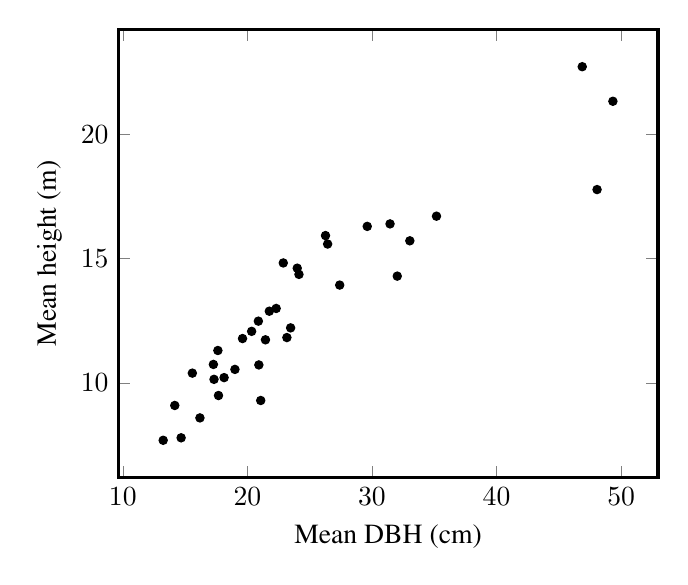
\begin{tikzpicture}
\tikzset{%%
  every mark/.append style={scale=1.0},%%
  scale=1.0%%
}
\pgfplotsset{%%
  every axis/.append style={font=\normalsize}%%
}
%%
\begin{axis}[%%
  axis line style=very thick,%%
  dotStyle/.style={mark size=1.5,black,mark color=black,mark=*,only marks},%%
  enlargelimits=true,%%
  %% x axis
  xlabel={\normalsize Mean DBH~(cm)},%%
  %% y axis
  ylabel={\normalsize Mean height~(m)}%%
]
%%
%%
\addplot[dotStyle] coordinates {
  (16.19, 8.6)
  (31.45, 16.4)
  (14.17, 9.1)
  (14.68, 7.8)
  (20.88, 12.49)
  (49.34, 21.33)
  (17.63, 11.31)
  (15.58, 10.4)
  (32.03, 14.3)
  (20.34, 12.08)
  (22.88, 14.83)
  (13.24, 7.7)
  (29.62, 16.3)
  (48.07, 17.78)
  (17.27, 10.75)
  (26.27, 15.93)
  (23.17, 11.83)
  (26.44, 15.59)
  (23.47, 12.22)
  (19, 10.55)
  (17.32, 10.15)
  (20.92, 10.73)
  (17.68, 9.5)
  (21.76, 12.89)
  (22.31, 13)
  (24, 14.62)
  (35.18, 16.71)
  (33.04, 15.72)
  (24.14, 14.37)
  (27.41, 13.94)
  (18.13, 10.22)
  (19.61, 11.79)
  (46.88, 22.72)
  (21.45, 11.74)
  (21.07, 9.3)
};
\end{axis}
\end{tikzpicture}

\end{document}
